\documentclass[12pt,letter]{article}
\usepackage{amssymb,microtype,tikz, amsmath, hyperref,setspace,todonotes}
\usepackage[T1]{fontenc}
\usepackage{color,parskip,siunitx,physics,marginnote}
\DeclareMathAlphabet{\mathscr}{OT1}{pzc}{m}{it}
\usepackage{epsfig, graphicx,subcaption,caption}
\usepackage{verbatim,marginfix}
\captionsetup[widefigure]{size = \textwidth}
\renewcommand{\footnotesize}{\scriptsize}
%\usepackage{mparhack}
\usepackage[driver=xetex,inner=2cm, outer=6cm, marginparsep=.5cm, marginparwidth=5cm, 
twoside=true]{geometry}
\usepackage[maxfloats=45]{morefloats}
\newcommand{\marginparstyle}{\footnotesize} % initialize style with start value
  \renewcommand*{\marginfont}{\marginparstyle}
\let\oldmarginpar\marginpar
\renewcommand*{\marginpar}[1]{\oldmarginpar{\begin{singlespace*} \marginparstyle #1
\end{singlespace*}}}
\usetikzlibrary{shapes.geometric, arrows}
\usepackage{sidenotes}
\usepackage{booktabs,adjustbox}
\title{Laser-Wakefield Electron Accelerators}
\author{Adam A. S. Green}
\begin{document}
\bibliographystyle{plain}
\maketitle
\doublespacing
\strictpagecheck

\begin{abstract}
In the late 1970's, Tajima and Dawson proposed a method of accelerating 
electrons using the large electric field gradients that plasmas are capable of 
sustaining. They showed that when a large amplitude laser pulse is sent through 
a plasma it can create a co-propagating longitudinal plasma wave 
capable of having electric field gradients of multiple
\si{\giga\electronvolt\per\centi\meter}-- orders
of magnitude larger than that of conventional particle accelerators.

In this work, we review the state-of-the-art experimental progress being made 
in creating a fully functioning electron accelerator based on laser plasma 
acceleration (LPA) technology. We discuss how the energy in an 
 electric field of a high intensity pulsed laser can be converted 
into an electric field gradient that can be used to accelerate electrons. 
We will review the physics of the laser-plasma interaction, and discuss the
limitations involved. We will finish with a review of the two most advanced
experimental efforts to advance LPA technology.  \end{abstract}
\tableofcontents
\section{Introduction}
\label{sec:intro}
The field of laser plasma acceleration is motivated by the goal of having
table-top electron accelerators capable of producing electron beams with
hundreds of \si{\giga\electronvolt}. This is achievable because the acceleration gradients that plasmas are capable of
sustaining are many orders of magnitude larger than conventional particle
accelerator. Much like the introduction of the personal computer in the era of massive
supercomputers, LPWA will put the technology of electron acceleration to
large energies in the hands of many.

 
 
 The ability to accelerate particles to high energies is a cornerstone
 in many areas of science. Although the recent discovery of the Higgs
 boson\cite{atlas} at the LHC demonstrated the value of ion-accelerators capable of
 TeV energies, a more direct comparison to the regimes achievable to LPWA
 technology would be to linacs-- such as Stanford Linear Accelerator Center
 (SLAC), which can excite electrons up to 50 \si{\giga\electronvolt}.

 Although historically important to the development of particle
 physics the most broad application of linacs such as SLAC is the use of
 accelerated electrons for an free-electron x-ray laser; the development of
 which has allowed investigation of structures from biology to solid state
 physics, as well as pioneering techniques in medical imaging.\cite{o2001free}
 

 But, much like the supercomputers of the 80's, the future of the field is limited by the size and expense of these
 facilities\sidenote{The famous cancellation of the Superconducting Super
 Collider in Texas due to budget problems in one dramatic example}. Laser plasma
 wakefield accelerators offer an option that is compact, and inexpensive by
 comparison. Although LPWA will never supplant linac's\sidenote{This is because
     the beam produced by LPWA is not continuous; the nature of LPWA schemes
     means that the electrons beam produced will be an intense bunch, rather
 than a continuous beam like SLAC.} they offer a complimentary approach at a
 fraction of the cost and real-estate. The prospect of a table-top free-electron
 laser has sparked intense interest in the field of laser plasma acceleration,
 and there is a dynamic field that is constantly improving the quality of the
 accelerated electron beam.


 The quest to produce high-energy electrons has four main goals: getting
  high-energy electrons; having a narrow energy distribution; producing collimated beams; and having a large number of electrons
 produced.

 In the context of free-electron lasers, these are important for the following
 simple reasons: the frequency of the x-rays scales with the square of the
 energy of the electrons, so the higher the energy the smaller length scales we
 can probe; the narrower the electron energy distribution, the narrower the
 x-ray linewidth; and the beam quality (number of electrons and angular spread)
 will also directly effect the x-ray laser coherence.
 \subsection{History}
 In the 1970's, Tajima and Dawson proposed shooting a high-intensity laser at a
 plasma\cite{PhysRevLett.43.267}. They predicted that the laser would generate a wakefield very similar to a boat moving
 through water and electrons could be accelerated by the wakefield.
  Unfortunately, the lasers of the day were unable to get
 to the high-intensities required. It was only the invention of the
 chirped-pulse laser (CPA) fifteen years later that allowed serious progress in
 the LPA field to occur\cite{backus1998high}.
\begin{marginfigure}
	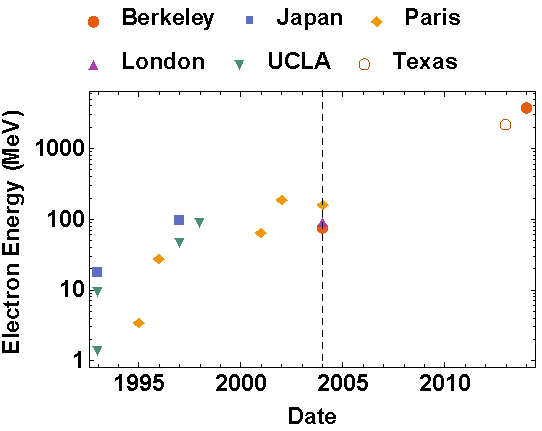
\includegraphics[width=\marginparwidth]{../figures/datfig.pdf}
    \caption{\label{fig:progress}The progress of laser plasma wakefield acceleration by the total
    energy of the electrons. The dashed line shows the advent of
    quasi-monoenergetic electrons, until that point the electron bunches had
    large thermal tails. \em This data was gathered from the web of science
abstract list}
\end{marginfigure}
In order to excite the plasma wave, you had to use a laser at the resonant
frequency, which scales with the square-root of the plasma density. For typical
laboratory plasmas, this resonant frequency was out of reach for the laser's of
the time. Several LPA schemes were devised to overcome
this, the two major ones being the plasma beatwave accelerator (PBWA), and the
self-modulated laser. Although the mechanics of these schemes differed the
underlying principle was to use the beatwave generated by spatio-temporally
overlapping two lasers to excite the plasma. This effort was moderately
successful: in 1995 electrons were successfully accelerated to energies in excess
of \SI{40}{\mega\electronvolt}. Unfortunately, these electron beams had large
Maxwellian energy distributions, making them untenable for practical
applications.

 In 2002, Pushkin predicted the bubble regime, which would solve many of the
 problems historically faced by LPWA schemes. By using a laser so powerful it
 completely expels electrons from a region, the bubble regime was predicted to
 be able to produce mono-energetic electron energies. However, it would require
 the discovery and development of CPA technology that would allow lasers to
 reach the intensities required to bubble.
 

 In 2004, this approach bore fruit, as three papers published simultaneously in
 Nature\cite{mangles2004monoenergetic,faure2004laser,Geddes2004}, demonstrated
 quasi-monoenergetic electron bunches in the bubble regime. Their results were
 soon extended to achieve energies of \SI{1}{\giga\electronvolt} in 2006
 \cite{Leemans2006}. 
 
 In 2013, a group at UT Austin produced a collimated, quasi-monoenergetic
 electron beam at 2.3 GeV\cite{Wang2013}, and in 2014 the Esarey group at UC
 Berkeley produced a 4 GeV\cite{PhysRevLett.113.245002} beam. These recent
 developments bring the field within striking distance of the LCLS at SLAC,
 which uses electrons accelerated to \SI{17.4}{\giga\electronvolt}.

 In the following section, we will discuss the physics of
 Laser-Plasma-Acceleration, and then discuss the two most recent experiments
 from UT Texas and UC Berkeley.
\section{The Physics of Laser-Plasma-Acceleration}
\begin{marginfigure}
    \resizebox{.7\marginparwidth}{!}{
    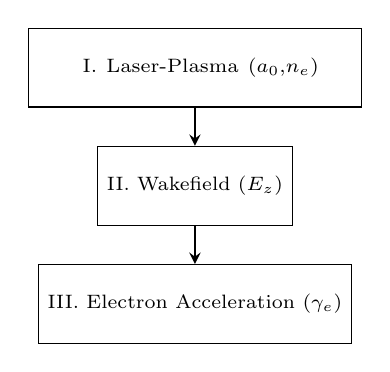
\begin{tikzpicture}[scale =.5,node distance = 1.5cm,auto]
        \node[draw,rectangle,minimum height=1cm,minimum width=2cm,text
        centered, text width = 4 cm,name=input]
        {\footnotesize \setstretch{1} I. Laser-Plasma ($a_0$,$n_e$)\\};
        \node[draw, rectangle, text centered, minimum height=1cm, minimum
        width=2cm, below of=input] (wakefield) {\footnotesize II. Wakefield ($E_z$)};
        \node[draw, rectangle, minimum height=1cm, text centered, minimum
        width=2cm, below of=wakefield] (eaccel) {\footnotesize III. Electron
        Acceleration ($\gamma_e$)};
        \draw  [thick,->,>=stealth] (input) -- (wakefield);
        \draw  [thick,->,>=stealth] (wakefield) -- (eaccel);
    \end{tikzpicture}
}
\caption{\label{fig:flow}The LWFA process. }
\end{marginfigure}
   
The LPWA process can be divided into three main topics, as shown in Figure
\ref{fig:flow}. First the intense laser (characterized
by the normalized field strength ($a_0 = e\vb{A}/m_e c^2$) interacts with the
plasma (characterized by the plasma density ($n_e$) producing a longitudinal
density modulation; this gives rise to a longitudinal electric field ($E_z$);
which will in turn accelerate the electrons to a relativistic energy
$\gamma_e$.This section will review each in turn.

Due to the complicated nature of the theory of LPWA in 3D relativistic fields, we will mainly
discuss these topics in the linear regime, and show the numerical results of
their extension into the 3D relativistic regime.

\subsection{Laser-Plasma Interaction}
 The interaction of the exciting laser
pulse with the plasma is governed by Lorentz force\cite{jackson}. As the
mass of the ions in the plasma is many orders of magnitude larger than the
electrons, it is valid to approximate the behaviour of the plasma as a fluid of
mobile electrons against a background of ions.

With this simple picture, the motion of the electrons will be governed by the
Lorentz force law, the continuity equation and Poisson's equation. If the
intensity of the laser is small enough, then these equations can be
liberalized, and are referred to the cold-fluid
equations\cite{gorbunov1987excitation}.
In this electron-fluid regime, the Lorentz force looks like:
\begin{align}
    \label{eq:fullLPWA}
    \pdv{\vb{p}}{t} +(\vb{v} \cdot \grad)\vb{p} = e \qty( \grad \Phi
    +\pdv{\vb{A}}{t} - \vb{v}\times \grad \times \vb{A} )
\end{align}

Where $\vb{p}$, $\vb{v}$ are the electron's momentum and velocity, and $\Phi$
and $\vb{A}$ are the scalar and vector potentials of the total field.

To first order, the movement of this fluid will be dominated by the force of the
electric field of the laser on the electrons, accelerating them in the polarization
plane. This is called the `quiver` momentum\footnote{So named because the electron will
undergo rapid oscillations while its time averaged acceleration will be zero, so it will appear to be quivering}. This quiver momentum will not produce a net acceleration on the 
electrons.

If the Lorentz force law is expanded out to second order, a term will appear that is
proportional to the intensity gradient, known as the ponderomotive force. This can be
thought of as the radiation pressure of the laser pulse, and will act to push
electrons away from the local space of the laser packet. It is this
ponderomotive force that will be directly used to drive the density waves that
all LPA schemes use. This is analogous to the physical situation of shooting a
cannonball underwater-- it will excite a density wave that co-propagates with
it.

By combining the Lorentz force with Possion's equation and the
fluid-continuity equation, a closed set of equations in one dimension can be found and solved to
give the behaviour of the plasma electrons:
\begin{equation}
    \label{eq:wave}
    \qty( \pdv[2]{t} + \omega_\mathrm{p}^2 ) = c^2 \laplacian \frac{a^2}{2}
\end{equation}
where we have introduced the normalized vector potential $a = eA/m_e c$, and the
resonant frequency of the electron fluid:
\begin{equation}
    \label{eq:wp}
    \omega_\mathrm{p} = \sqrt{\frac{e^2 n_e}{m_e \epsilon_0}},
\end{equation}
Where $m_e$, $n_e$, and $e$ are the mass, density and charge of the electron, respectively.

The resonant frequency of the plasma will give an experimental constraint. As
with all driven-oscillator type systems, to drive the oscillator at resonance,
you need to force it at the natural frequency of the system. We want
high-intensity waves, as their amplitude will ultimately determine the
accelerating field $E_z$. In order to excite resonance then $\tau_\textrm{laser}
\omega_p \approx \pi$. The resonance condition is further illustrated in Figure
\ref{fig:resonance}.
In this regime, the density of the electrons behaves like a wave that
co-propagates with the laser pulse. We can connect the variations in density to
the electric field produced using Possion's equation, which reduces to
\begin{equation}
    \vb{k}\dotproduct\vb{E} = \frac{\delta n_e}{\epsilon_0}
\end{equation}
This shows there will be a co-propagating electric field, which points along
the propagation direction, and oscillates $\pi$ out of phase from the density
w
This field $E_z$ is the one that will be used to accelerate electrons.
This process can be generalized into a non-linear regime by simply eliminating
the assumption that $a \ll 1$, and an analytic solution can be found. However, in three
dimensions the equations become intractable and numerical simulation is
required to solve them. The solutions in one-dimension are plotted in Figure \ref{fig:plasmon}
for a range of parameters.
\begin{figure}[h!]
        \begin{singlespace*}
        \centering
        \begin{subfigure}[t]{\textwidth}
            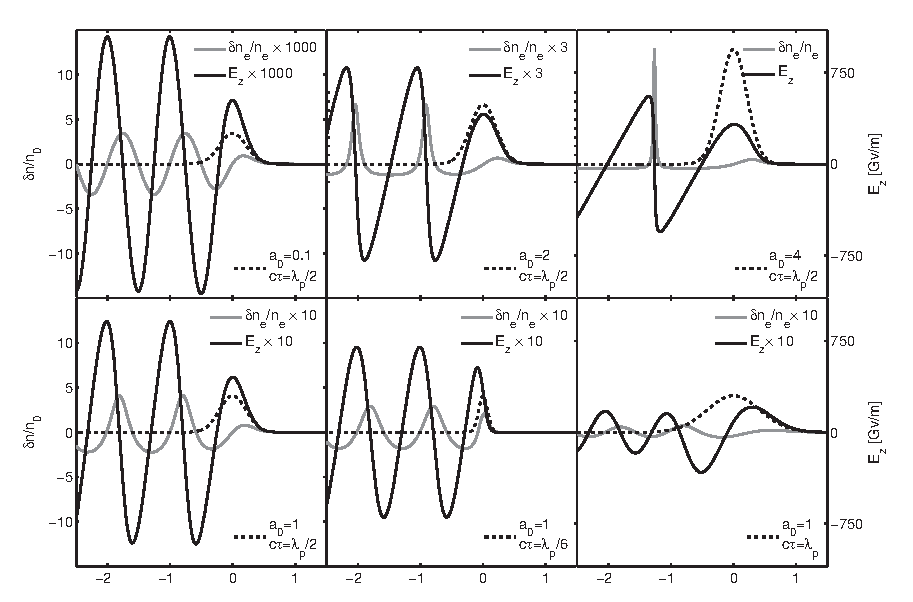
\includegraphics[height = .4\textheight]{../figures/densityandewave.eps}
            \caption{\small  Showing plasmons generated with varying strengths of the peak
                amplitude of the laser pulse.\cite{genothesis}\label{fig:plasmon}
                The laser pulse is the dashed line, the density perturbation is the grey
                line, and the longitudinal electric field $E_z$ is the black
                curve. The x-axis is showing the normalized co-ordinate $\zeta =
                kz - wt$, which shows the evolution of the phase-front. Different
                scenarios are shown: from left to right, the normalized field strength variable
                ($a = eA/m_e c^2$) is varied, and from top to bottom, the duration of
                the laser pulse is changed. \em Figure courtesy of Guillaume Genoud, Lund
            University}
        \end{subfigure}

        \begin{subfigure}[t]{\textwidth}
            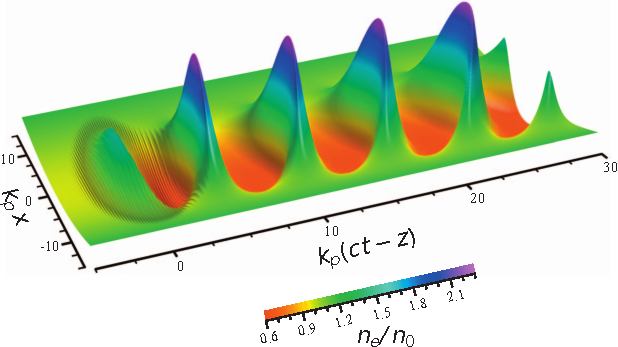
\includegraphics[height = .3\textheight]{../figures/esarey3dnonlin.pdf}

            \caption{\small  Numerical simulation for a 2D, non-linear model. Many of the
                features in the 1D model remain-- the signature `leaning' of the density
            pulse as it becomes non-linear being the most striking. }
        \end{subfigure}
\end{singlespace*}
    \end{figure}

It is worth noting that modern LWFA schemes operate in the bubble regime, where the laser pulse is so
intense that it completely expels the electrons from its local space-- putting
us firmly in the non-linear 3D regime.  This means that the 
majority of theoretical work currently being done is by using numerical methods.
An example is given in Figure \ref{fig:bubble}
\begin{marginfigure}[0pt]
    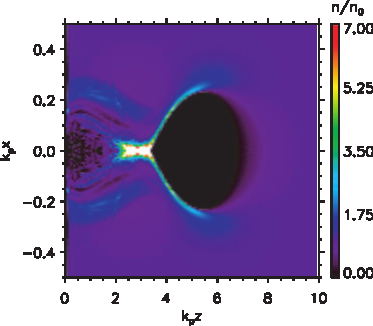
\includegraphics[width=\marginparwidth]{../figures/esblowout.pdf}
    \caption{\label{fig:bubble} An example of the bubble regime created by a laser pulse with $a =
    .3)$. The laser is moving toward the right.\cite{RevModPhys.81.1229}}
\end{marginfigure}

   \subsection{Electron Trapping, Injection, and Acceleration}

    In order to be accelerated by the co-propagating electric field created by the
    plasmon, the electrons need to be travelling at some minimum speed.
    Transforming to the rest-frame of the plasmon, only those electrons that are
    moving slowly enough will be trapped by the electrostatic field.
    The phase-space trajectories of various test electrons are shown in Figure
    \ref{fig:trapping}, illustrating that only for a specific range of the
    electron momentum will they actually be able to be trapped. The background
    electrons will not meet these requirements in the linear regime. This can be
    overcome by having an external injection source of electrons, but this has
    the obvious disadvantage of already requiring electrons with large energies.
    As we discuss below, there is a way to use accelerate the background
    electrons.
\begin{figure}[h]%
    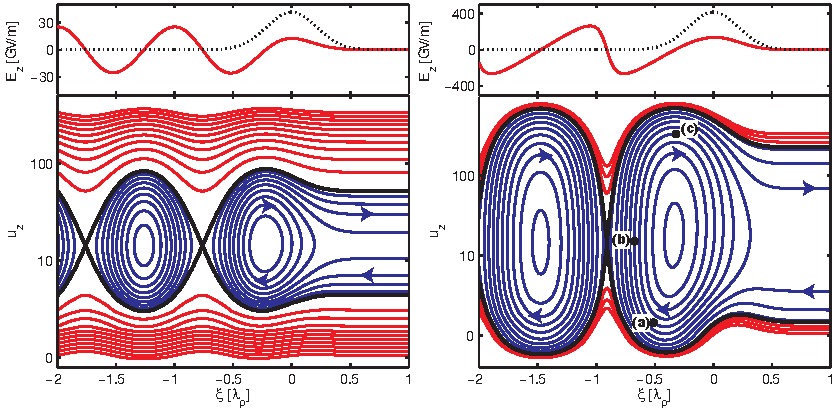
\includegraphics[width=\textwidth]{../figures/trapping.pdf}
    \caption{\label{fig:trapping} The various trajectories of electrons at
    different initial momentum ($u_z= p/m_e c^2$) in the reference frame of the laser
pulse, which is moving at an relativistic energy $\gamma = 13$ in the lab frame.
For specific initial electron energies the electrons will be trapped and
accelerated by the wakefield. }
\end{figure}


    If the amplitude of the laser field is strong enough to excite the plasmon into a non-linear regime, then there are ways for the background electrons to be
accelerated. This process is referred to as self-injection. \sidenote{Although self-injection happens in
        non-linear fields in both 1D and 3D, it occurs by different physical
    processes\cite{esatrap}. We will be focusing on the 3D case in this review}
    
    Looking at Figure \ref{fig:plasmons}, the
    non-linear regime plasmons are steeper on one edge. This is due to the fact
    that the background electrons are having enough energy imparted to them to
    affect the shape and properties of the plasmon. This process, referred to as
    wavebreaking, is useful for
    two reasons: it enhances the overall field and allows the background
    electrons to meet the velocity requirements to be trapped by the plasmon.
    The bubble regime, in which the laser is powerful enough to completely
    expel the electrons from a central region of the pulse, is an extreme
    example of wavebreaking in plasmons. Figure \ref{fig:bubbleschem} is a
    schematic of the bubble regime.

    \begin{marginfigure}[-70pt]
    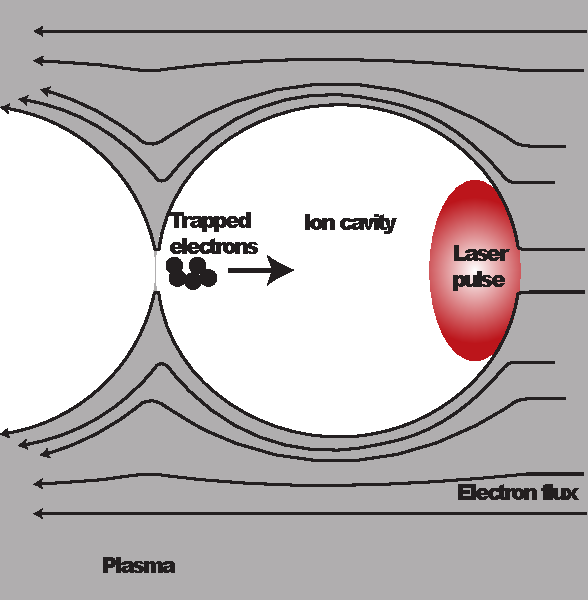
\includegraphics[width=\marginparwidth]{../figures/bubbleschem.pdf}
    \caption{A schematic of the bubble
    regime.\cite{genothesis}\label{fig:bubbleschem}}
\end{marginfigure}



    It can be shown using a combination of numerical and analytical analysis that in the bubble regime there is a specific requirement
    for the radius of the bubble for self-injection to occur:$R/\sqrt{2} >
    \omega_0/\omega_p$, where $R$ is the radius of the bubble, and $\omega_0$ is
    the laser frequency.\cite{PhysRevLett.103.175003}. 

    \begin{marginfigure}[70pt]
        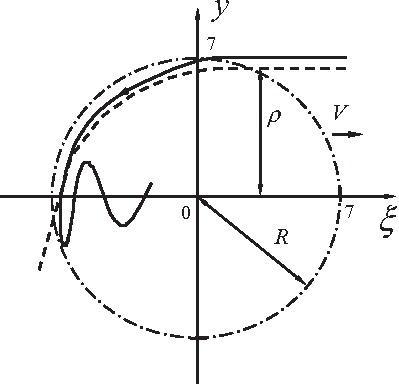
\includegraphics[width = \marginparwidth]{../figures/bubbletrap1.pdf}
        \caption{Showing a trapped, and untrapped trajectory of an electron. The
        bubble parameters are $R = 7$, $\gamma_0 = 4$}
\end{marginfigure}
    
However, it is easy to gain a phenomenological explanation of the dynamics of
self-injection in the bubble regime. The bubble can be thought of as an
ion-cavity moving relativistically through an
electron fluid. A small sheath of electrons will form as a boundary layer
between the ion-cavity and the surrounding electron fluid. This sheath will be
in contact with the relativistic fields of the cavity for the longest time, and
is the best candidate to be accelerated. If the laser defocuses, then the bubble
will grow. If it grows on a time scale that is quick enough, electrons that
previously wouldn't have the right initial orbit are now have a small enough
relative velocity to be trapped. Although the dynamics of the laser evolution in
the plasma are complicated, it will undergo cycles of focusing and defocusing
due to diffraction and self-focusing phenomena-- discussed in more detail in
Section \ref{sec:selffocus}. In this way, the bubble will breath, trapping and
accelerating electrons. 

\begin{margintable}[0pt]
    \resizebox{\marginparwidth}{!}{%
    \begin{tabular}{lccc}
        \toprule
        Model  & $L_d$ & $L_{pd}$ & $L_\textrm{diff}$ \\ \midrule
        Linear & $\frac{\lambda_d \omega_0^2}{\omega_p^2}$ & $\frac{c
    \omega_0^2\tau}{\omega_p^2 a_0^2}$& $\frac{\pi \lambda_p^2}{\lambda_0} $ \\
        Non-Linear & $\frac{4}{3} \frac{c \omega_0^2}{\omega_p^2}\sqrt{a_0}$&$
        \frac{c \omega_0^2\tau}{\omega_p^2}$ & $\pi
    \frac{ a_0 \lambda_p^2}{\lambda_0}$\\
    \bottomrule
\end{tabular}}
\caption{The scaling laws for limiting lengths in LPWA.}
\end{margintable}
    
    \subsection{Electron Acceleration}
    The plasma bubble will set up a very high \si{\giga \electronvolt \per
\centi \meter} acceleration field, however what will limit the total energy
    gain is how far the electron can be accelerated for. 
    We will discuss the scaling behaviour of the three length scales that
    dominate the laser-plasma
    interaction..
    

    The first, $L_\mathrm{Pulse Depletion}$, occurs because the interaction
    with of the laser-plasma will dissipate the energy of the initial laser
    pulse. The energy in the initial laser will be transfered to the plasma
    wake, where it will ultimately be dissipated as heat. In 1D, this can
    be approximated quite well by simply equating
    the total energy of the laser to the energy in the wakefield:
    $E_z^2L_{pd} = E_L^2L$, where $E_z$ is the wakefield and $E_L, \,L$ refer
    to the laser field and pulse length,
    respectively\cite{RevModPhys.81.1229}.

    In a non-linear 3D regime, an estimate based on the 1D non-linear was
    found to still be accurate. There the pulse depletion is given as the
    laser-front is etched away as it excites the wakefield. This etching
    velocity is given as $v_\textrm{etch}
    \approx c \omega_p^2 /w_0^2$ \cite{deckedevolv}. The pump depletion
    length is then given by:
    \begin{equation}
        L_\textrm{etch} \approx \frac{c}{v_\textrm{etch} c
            \tau_\textrm{FWHM}}
        \end{equation}


    The second, $L_\mathrm{Dephasing}$ is analogous to what happens
    when a surfer outruns the wave they are on; no longer being accelerated,
    they slow down as their energy is dissipated to the waves. Similarly, electrons
    can outrun the plasma bubble. In 1D, this concept can be simply defined
    as the length it takes for the electron's phase to slip by one-half
    of the plasmon. For the 3D theory theory in the bubble regime, a good approximation of this
can be found by estimating the electron's velocity as $c$, and asking
when it will overtake the bubble, which is moving at a slower velocity
$v_\phi-v_\textrm{etch}$. Solving this gives
\begin{equation}
    L_d \approx \frac{c}{c-v_\phi}R
\end{equation}
where $R$ is the bubble radius.
    The third length, $L_\mathrm{Diffraction}$ is the most important, as it is
    the limiting length scale. This length scale is due to the inherent
    diffraction of lasers. In order to achieve the intense energies necessary
    for the bubble regime, the lasers need to be focused down to a specific spot
    size. As soon as the minimum spot size is reached, the laser will begin to
    diffract, the length scale where the laser is approximately the spot size is
    the Rayleigh length. In a plasma this becomes more complicated, as the
    plasma can and will act like a lens. This leads to a feedback effect, where
    the intense laser pulse will change the plasma density, which in turn
    changes the intense laser pulse, and so on. The majority of effort in current wakefield accelerator  programs is to overcome this issue.

    In Figure \ref{fig:energy}, we can see the length scales multiplied by the
    accelerating electric field-- giving the total energy possible if an
    electron was accelerated over that distance. Clearly, the limiting length
    scale is diffraction.
    \begin{marginfigure}
            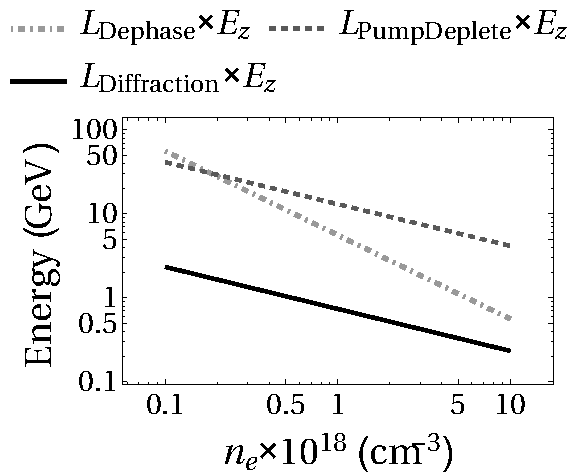
\includegraphics[width=\linewidth]{../figures/energy.pdf}
        \caption{The three length scales involved with accelerating electrons:
        $L_\mathrm{Dephase}$ where the electron outruns the wave, self-limiting
    the total energy gained; $L_\mathrm{Pump Depletion}$ where the incident
energy in the laser pulse is completely transfered to the wakefield, and the
laser can no longer sustain the bubble regime; and $L_\mathrm{Diffraction}$ the
inherent diffraction of the laser pulse. All lengths are scaled by an
accelerating field using parameters from the Texas
experiment\cite{Wang2013}, to show the total possible energy an electron
could gain.\label{fig:energy}}
    \end{marginfigure}

    There are several strategies for extending the length of the laser-plasma
    interaction: two that we will mention are relativistic self-focusing, and
    external plasma-waveguide solutions. These are the two main solutions
    currently being pursued by the UT Texas group and the Berkeley group,
    respectively.

\section{Experimental Set-Up and State-of-the-Art}
In this review, we will focus on the experimental efforts of two groups, UT
Austin Texas, and University of California Berkeley. Although there are many
more groups doing interesting work in the field of LWFA, these two groups are
the main ones actively pursuing the goal of high-energy electron
acceleration.

The Texas group uses very high-intensity laser pulses and exploits the
phenomena of relativistic self-guiding to cancel out the inherent diffraction
of the laser. The Berkeley group uses low-intensity laser pulses and plasma waveguide channels to overcome the diffraction issue. A more in depth review of
each group and method is presented below.

\subsection{Texas: Relativistic Focusing}

In 2013, the Texas group reported a collimated beam of \SI{2}{\giga
\electronvolt}, which blew current records out of the
water\cite{Wang2013}.

Their approach used the new petawatt laser facility at UT Austin. The large
amplitudes that the laser was capable of generating placed them firmly in the
relativistic self-guiding regime.

\subsubsection{Relativistic Self-Guiding}
The group velocity of the laser pulse will be set by the index of refraction of
the medium, which in turn is $eta = v_g/c = c^{-1}\dv{w}{k}$.  The dispersion
relation for a plasma is shown in Figure \ref{fig:disperion}. Thus,
\begin{equation}
    \label{eq:index}
    eta = \qty(1-\frac{\omega_p^2}{\omega^2})^{1/2}.
\end{equation}

If $eta$ has a density distribution where it is larger on the optical axis, then
a guiding plasma lens will be formed that can counteract the effects of
diffraction. As we will discuss below, one can use relativistic effects to
achieve this. 
\begin{marginfigure}
    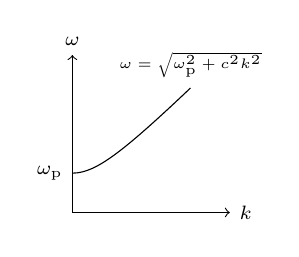
\begin{tikzpicture}[domain=0:4,scale=.5]
        \draw[->] (0,0) -- (4,0) node[anchor=west,font=\footnotesize] {$k$};
        \draw[->] (0,0) -- (0,4) node[anchor=south,font=\footnotesize] {$\omega$};
        \draw (0,1) node[anchor=east,font=\footnotesize] {$\omega_\mathrm{p}$};
        \draw[scale=1, domain = 0:3,smooth,variable=\x,black] plot ({\x},{sqrt(\x*\x+1)})
        node[above,font=\tiny] {$\omega = \sqrt{\omega_\mathrm{p}^2 + c^2 k^2}$};
\end{tikzpicture}
    \caption{\label{fig:dispersion}The plasma dispersion relation. We will be
        dealing with plasmas where $\omega_\mathrm{p}/\omega << 1$, so to
    first order the laser will be dispersionless. }
    \end{marginfigure}

Remembering back to Section \ref{sec:laser}, the first order effect of the
high-intensity laser pulse will make the electrons quiver in the polarization
plane.If the laser is intense enough, the electrons will be quivering
relativistically, and will have maximum energy as they pass through the optical
axis of the pulse. This means that their mass will be a maximum on the optical
axis. This can be roughly seen to change the index of refraction, as:
\begin{equation}
    \label{eq:indexrel}
    \eta(m_e) \rightarrow \eta(\gamma m_e) \approx
1-\frac{\omega_p^2}{2\omega^2}\frac{\delta n(r)}{\gamma}
\end{equation}
where $\delta n(r) $is a density variation, and $gamma$ will be a maximum on
axis.\cite{esarey} This gives rise to the focusing behaviour
discussed above.

This sets a very harsh experimental parameter, as the fields have to be
relativistic enough to be able to counter the effects of diffraction. It can be
shown that this limit is that the power in the field is P(GW) = 17.4
$(\omega/\omega_p)^2$\cite{esarey}.

In reality, the dynamics are much more complicated, and require detailed
numerical simulations, one such example is shown in Figure
\ref{fig:propsim}\cite{Wang2013}. This is partially due to the fact that the
front and back of the waves will not satisfy the relativistic criterion, and
diffract away-- dynamically changing the pulse shape, which can have an effect.
\begin{marginfigure}
	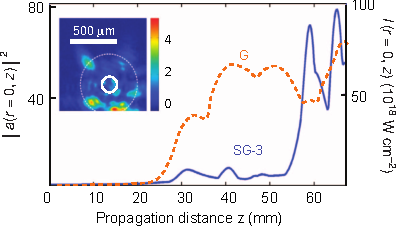
\includegraphics[width=\marginparwidth]{../figures/wakesimulation.pdf}
    \caption{Simulations done by the Texas group using the WAKE
        code showing clear features of self-focusing.\cite{Wang2013} As the
        normalized laser-intensity gets larger, the pulse is
        contracting--concentrating more of its energy over a smaller area.
        Interestingly, the self-focusing exhibits a periodic structure-- going
        through two cycles of diffraction-focusing for the super-Gaussian
    pulse.\label{fig:propsim}}
\end{marginfigure}

\subsubsection{Experimental Setup and Results}
Shown in Figure \ref{fig:experTexas} is the experimental setup for Texas. At
its heart, it is a high-intensity laser that is hitting an ionized gas. The
majority of the experiment is the diagnostics, which allow the team to determine
the energy and spread of the electrons.
\begin{figure}[b!]
	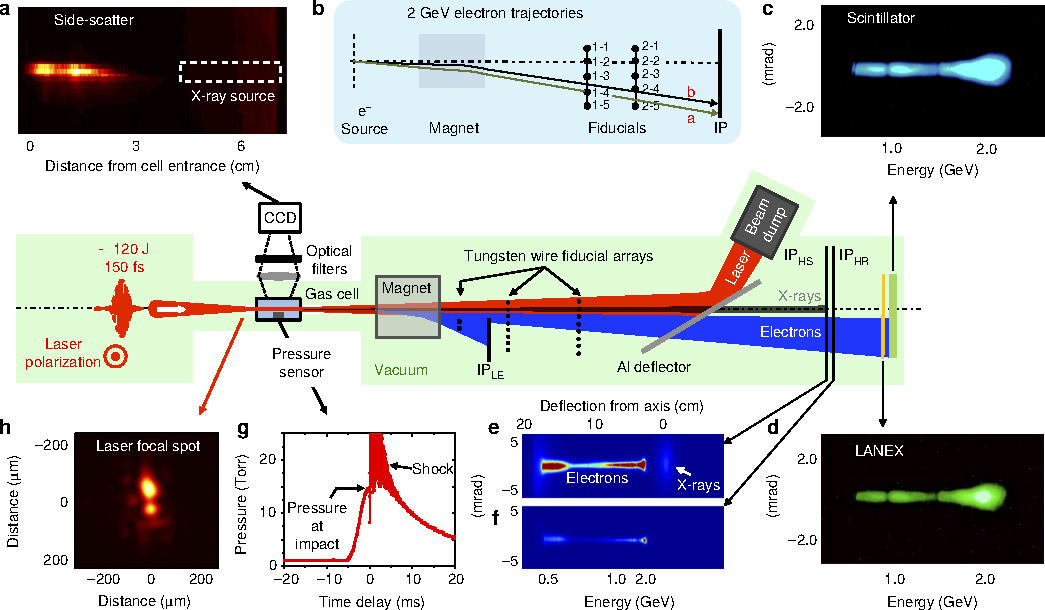
\includegraphics[width=\textwidth]{../figures/texasexplayout.pdf}
    \caption{\small The experimental setup of the Texas group.\cite{Wang2013}
        {\em This
        figure is reproduced from Nat. Commun. Vol. 4, 2013. } The laser hits
            a gas cell. It will propogate in the plasma, until the self-focusing
            process reaches a critical point, where the laser-plasma will enter
            the bubble regime. \textbf{a)} Detector to measure sidescatted light
            from gas-laser interaction. \textbf{b} Schematic showing how the
            electrons are bent using a magnet-- acting like a spatial filter for
            momentum. There are tungsten posts that will cast `shadows' on the
            electron detector, allowing the source of the electrons to be
            backtracked. \textbf{c} Electron spectrum on the scintillator.
            \textbf{d} Another spectrum on the LANEX. \textbf{e)\&f)} X-ray beam
            blocker. \textbf{g} Pressure sensor on the gas cell. \textbf{h}
            Image of the laser spot-size.
        \label{fig:experTexas} }
    
\end{figure}

The Texas group is now hard at work trying to find a strategy to increase the
energy of the electrons. This is due to the very complicated dynamics of the
highly non-linear laser-plasma interaction that leads to self-focusing. As
shown in Figure \ref{fig:propsim}, the behaviour of the self-focusing is very
dependent on initial conditions (laser intensity, laser pulse shape, etc.). As
no analytic model can fully encompass its behaviour, numerical simulation is
required to understand the self-focusing behaviour required to produce
acceleration lengths required for high energy electrons.

\subsection{Low-Intensity, Quasi-Linear Plasmas with Waveguides}

\begin{marginfigure}
    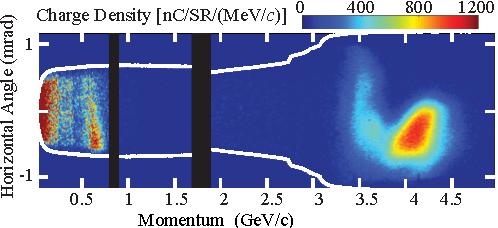
\includegraphics[width=\marginparwidth]{../figures/esaenergy.pdf}
    \caption{The energy spectrum for the recent Berkeley result.}
\end{marginfigure}


In 2014, the Berkeley group reported a collimated electron beam with peak
energy of \SI{4.2}{\giga \electronvolt}.

The Berkeley has, for a while now, pursued the strategy of low-intensity laser
pulses that are guided through channels. Their most current results use a
capillary discharge channel. The physics of focusing remain the same: there is a
radial density profile that has the same profile as a focusing lens. Instead of
the density profile coming from relativistic effects, like the Texas group, the
Berkeley group uses a plasma channel guide, which is a simple tube containing
hydrogen gas, with a metal plate at each end. A voltage is applied across the
length of the tube, ionizing the gas. The gas will cool down more rapidly along
the edges of the tube, and this will give rise to an approximately parabolic
density profile of the hydrogen
gas\cite{PhysRevLett.89.185003,PhysRevE.63.015401}. It is this parabolic density profile which
will act as the focusing lens of the plasma wave. The evolution of a laser pulse
in a plasma channel is shown in Figure \ref{fig:esasim}. 
\begin{marginfigure}
	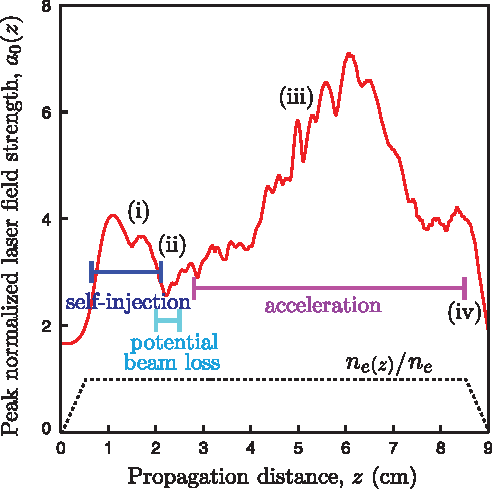
\includegraphics[width=\marginparwidth]{../figures/esareycapfield.pdf}
    \caption{Evolution of the peak normalized intensity of the laser pulse,
    ($a_0(z)$ done using a particle-in-cell simulation for a top-hat laser pulse
    with energy 16 J, through a 9 \si{cm} plasma waveguide. {\em From Leemans
et. al. 2014 \cite{PhysRevLett.113.245002}}\label{fig:esasim}}
\end{marginfigure}


The benefits over the Texas strategy is that they gain significantly on energy
conversion.  The use of the plasma channel makes the laser-wakefield interaction
more stable, the pulse takes much longer to diffract-- allowing the electrons to
be accelerated over a much larger distance. This means that a lower intensity
laser can be used. 
 As well, there are some concerns in the field
that the relativistic self-focusing process is too unstable to guide the beam
over the necessarily distances\cite{RevModPhys.81.1229}, but some progress has
been made to extend the distances that relativistic self-guiding can be used
over\cite{PhysRevLett.113.245001}.


\section{Conclusion}
In this review, we have highlighted two approaches for electron acceleration:
the high-intensity, relativistically guiding approach used by Texas, and the
low-intensity, plasma-channel guided approached used by Berkeley. For further
progress to be made in the field, there needs to be a better understanding of
the evolution of the laser-plasma interaction and evolution. It is worth noting
that the bubble regime-- the regime used by all groups trying to achieve GeV
acceleration-- was first seen in simulations. 

New imaging techniques at UT Texas, which allow in vivo imaging of the evolution
of the laser and plasmon, as well as novel theoretical and computational
approaches are the current frontier. The raw power exists to accelerate
electrons to high GeV energies, all we need to do is control it.
\bibliography{../rep.bib}
\end{document}

